\documentclass{beamer}
\usepackage{xeCJK}
\setCJKmainfont{STXIHEI.TTF}

%
% Choose how your presentation looks.
%
% For more themes, color themes and font themes, see:
% http://deic.uab.es/~iblanes/beamer_gallery/index_by_theme.html
%
\mode<presentation>
{
  \usetheme{Warsaw}       % or try Darmstadt, Madrid, Dresden, ...
  \usecolortheme{default} % or try albatross, beaver, crane, ...
  \usefonttheme{default}  % or try serif, structurebold, ...
  \setbeamertemplate{navigation symbols}{}
  \setbeamertemplate{caption}[numbered]
} 

\usepackage[english]{babel}

\title{尚书·牧誓}
\author{周武王}
\institute{商郊牧野}
\date{甲子昧爽}

\begin{document}

\begin{frame}
  \titlepage
\end{frame}

\begin{frame}{目录}
  \tableofcontents
\end{frame}

\section{提纲}

\begin{frame}[fragile]{\insertsection}

\begin{itemize}
  \item 大家都来了 (辛苦了;注意听讲)
  \item 商纣王——太差劲了
  \item 要团结(形势险恶)
\end{itemize}

\end{frame}

\begin{frame}{备忘录!}

\begin{itemize}[<+->]
  \item 我们人不多
  \item 先点名
  \item 记住讲稿
\end{itemize}

\end{frame}

\section{回顾}

\begin{frame}{主要目的 \& 取胜要素}

\begin{itemize}
\item 纣王要害:
  \begin{itemize}
    \item  无贤才
    \item 失民心
  \end{itemize}
\end{itemize}

\begin{block}{战场军风:}
\begin{itemize}
\item 桓桓如虎
\item 如貔
\item 如熊
\item 如罴
\end{itemize}
\end{block}

\end{frame}

\begin{frame}{组织结构}

\begin{figure}
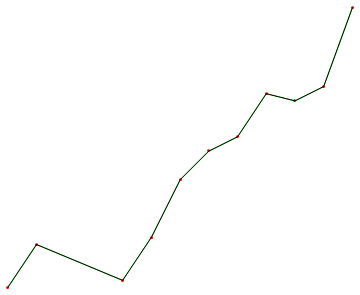
\includegraphics[width=0.5\textwidth]{Splines-1.png}
\end{figure}

\begin{block}{千夫长,百夫长}
\begin{equation}
\frac{1000}{100}=10\times 1
\end{equation}
\end{block}

\end{frame}

\section{Summary}

\begin{frame}{总结}

\begin{columns}
\begin{column}{0.6\textwidth}
\begin{itemize}
\item 必须赢得战争
\item 否则会被杀戮
\end{itemize}
\end{column}
\begin{column}{0.4\textwidth}
\begin{itemize}
\item 前进吧
\item 勖哉夫子
\end{itemize}
\end{column}
\end{columns}

\end{frame}

\end{document}

